%!TEX root = popl2018.tex

\section{Decision procedure for $\strline[\replaceall]$: The constant-string case}\label{sec:replaceallcs}

In this section, we consider the constant-string special case, that is, for an $\strline[\replaceall]$ formula $C = \varphi \wedge \psi$, every term of the form $\replaceall(z, e, z')$ in $\varphi$ satisfies that $e=u$ for $u \in \Sigma^+$. Note that the case when $u=\epsilon$ will be dealt with in Section~\ref{sec:replaceallre}. 

Again, let us start with the simple situation that
$$C \equiv x = \replaceall(y, u, z) \wedge x \in e_1 \wedge y \in e_2 \wedge z \in e_3,$$
where $|u| \ge 2$. For $i=1,2,3$, let $\cA_i = (Q_i, \delta_i, q_{0, i}, F_i)$
be the NFA corresponding to $e_i$. In addition, let $k = |u|$ and $u = a_1 \cdots a_k$ with $a_i \in \Sigma$ for each $i \in [k]$.

According to the semantics, $C$ is satisfiable iff $x, y, z$ can be assigned with  strings $v, w, w'$ such that: (1) $v = \replaceall(w, u, w')$, and (2) $v,w, w'$ are accepted by $\cA_1, \cA_2, \cA_3$ respectively. Let $v, w, w'$ be the strings satisfying these two constraints. Since $v = \replaceall(w, u, w')$, we know that there are strings $w_1, w_2, \cdots, w_n$ such that $w= w_1 u w_2 \cdots u w_n$ and $v = w_1 w' w_2 \cdots w' w_n$. As $v$ is accepted by $\cA_1$, there is an accepting run of $\cA_1$ on $v$, say
$$
q_{0,1} \xrightarrow[\cA_1]{w_1} q_1 \xrightarrow[\cA_1]{w'} q'_1 \xrightarrow[\cA_1]{w_2} q_2 \xrightarrow[\cA_1]{w'} q'_2 \cdots q_{n-1} \xrightarrow[\cA_1]{w'} q'_{n-1} \xrightarrow[\cA_1]{w_n} q_n.
$$
Let $T_z = \{(q_i, q'_i) \mid i \in [n]\}$. Then $w' \in \Ll(\cA_3) \cap\ \bigcap \limits_{(q,q') \in T_z} \Ll(\cA_1(q, q'))$. Therefore, $\Ll(\cA_3) \cap\ \bigcap \limits_{(q,q') \in T_z} \Ll(\cA_1(q, q')) \neq \emptyset$. Similar to the single-letter case, we will construct an NFA $\cB_{\cA_1, u, T_z}$ to characterise the satisfiability of $C$.  More precisely, $C$ is satisfiable iff there is $T_z \subseteq Q_1 \times Q_1$ such that $\Ll(\cA_3) \cap\ \bigcap \limits_{(q,q') \in T_z} \Ll(\cA_1(q, q')) \neq \emptyset$ and
$\Ll(\cA_2) \cap \Ll(\cB_{\cA_1, u, T_z}) \neq \emptyset$. Intuitively, when reading the string $w$, $\cB_{\cA_1, u, T_z}$ simulates the generation of $v$ from $w$ and $w'$, that is, simulates the replacement of  every occurrence of $u$ in $w$ with $w'$, and verifies that $v$ is accepted by $\cA_1$, by using $T_z$.
The construction of $\cB_{\cA_1, u, T_z}$ utilises the concepts of window profiles and parsing automata defined below.
%
%Intuitively, the window profiles encode the matching of the suffixes of a string of length $|u|$ w.r.t. the prefixes of $u$ and a parsing automaton for $u$ uses window profiles of $u$ to pinpoint the first, second, \dots, occurrence of $u$ in a string.


%Let us start with the simple case that $C \equiv x = \replaceall(y, u, z) \wedge \bigwedge \limits_{i \in [k]} x \in e_{i}$ such that $|u| \ge 2$.  In addition, for $i \in [k]$, suppose $\cA_i = (Q_i, \delta_i, q_{0, i}, F_i)$
%is the NFA corresponding to $e_i$.
%\begin{enumerate}
%\item For each $i \in [k]$, we will guess a set $T_{i, z} \subseteq Q_i \times Q_i$, which intuitively means that in $\cA_i$, for each state pair $(q, q') \in T_{i, z}$, starting from $q$, after reading $z$, the state $q' $ can be reached. The functions $(T_{i, z})_{i \in [k]}$ induce regular constraints $\Ll(\cA_i(q,q'))$ on $z$, where $i \in [k]$ and $(q,q') \in T_{i, z}$.
%
%\item For each $i \in [k]$, we construct an NFA $\cB_{\cA_i, u,  T_{i, z}}$, which specifies some additional regular constraint on $y$. Intuitively, a string $v$ is accepted by $\cB_{\cA_i, u,  T_{i, z}}$ iff either $v \not \in \Sigma^\ast u \Sigma^\ast$ and $v$ is accepted by $\cA_i$, or otherwise, let $v = v'_1 u v'_2 u \dots v'_{k-1} u v'_{k}$ such that $v'_i u' \not \in \Sigma^\ast u \Sigma^\ast$ for each $i \in [k-1]$ and each strict prefix $u'$ of $u$ and $v'_k \not \in \Sigma^\ast u \Sigma^\ast$, then $q_{i,0} \xrightarrow{v'_1} q_1 \xrightarrow{T_{i,z}} q'_1 \xrightarrow{v'_2} q_2 \xrightarrow{T_{i,z}} q'_2 \dots \xrightarrow{v'_{k-1}} q_{k-1} \xrightarrow{T_{i,z}} q'_{k-1} \xrightarrow{v'_k} q_k$ for states $q_1, q'_1, \dots, q_{k-1}, q'_{k-1}, q_k \in Q_i$ with $q_k \in F_{i,z}$.
%\end{enumerate}
%
%In order to construct the NFA $\cB_{\cA_i, u,  T_{i, z}}$, we introduce concepts of window profiles and parsing automata defined below.
%
%Let $u \in \Sigma^+$ and $k=|u| \ge 2$.


\begin{definition}[$k$-window profiles w.r.t. $u$]
Let $v$ be a nonempty string and $i \in [|v|]$. Then the $k$-\emph{window profile of the position $i$ in $v$ w.r.t. $u$} is $\overrightarrow{W}  \in \{\bot,\top\}^{k-1}$ defined as follows:
\begin{itemize}
\item If $i \ge k-1$, then for each $j \in [k-1]$, $\overrightarrow{W}[j] = \top$ iff $v[i-j+1] \cdots v[i]=u[1] \cdots u[j]$.
%
\item If $i < k-1$, then for each $j \in [i]$, $\overrightarrow{W}[j] = \top$ iff $v[i-j+1] \cdots v[i]=u[1] \cdots u[j]$, and for each $j: i < j \le k-1$, $\overrightarrow{W}[j] = \bot$.
\end{itemize}
Let $\wprof_{u, k}$ denote the set of $k$-window profiles of the positions in nonempty strings w.r.t. $u$.
\end{definition}

%Intuitively, in a position $i$ of a string $v$, the $k$-window profile $\overrightarrow{W}$ of $i$ in $v$ w.r.t. $u$ is an abstraction of the substring $v[i-k+2] \dots v[i]$ such that for each $j \in [k-1]$, $\overrightarrow{W}[j] = \top$ iff $v[i-j+1] \dots v[i] = u[1] \dots u[j]$.

\begin{proposition}
$|\wprof_{u,k}| \le k$.
\end{proposition}
%
\begin{proof}
%The arguments for this fact proceed as follows: 
For each profile $\overrightarrow{W}$, let $v$ be a nonempty string and $i$ be a position of $v$ such that for each $j \in [k-1]$, $\overrightarrow{W}[j] = \top$ iff $v[i-j+1] \dots v[i] = u[1] \dots u[j]$. Define ${\sf idx}_{\overrightarrow{W}}$ as follows: If there is $j \in [k-1]$ such that $\overrightarrow{W}[j]=\top$, then ${\sf idx}_{\overrightarrow{W}}$ is the maximum of such indices $j \in [k-1]$, otherwise, ${\sf idx}_{\overrightarrow{W}} =0$. The following fact holds for $\overrightarrow{W}$ and ${\sf idx}_{\overrightarrow{W}}$: 
\begin{itemize}
	\item for each $j': {\sf idx}_{\overrightarrow{W}} < j' \le k-1$, $\overrightarrow{W}[j']=\bot$,
	\item in addition, since $v[i-{\sf idx}_{\overrightarrow{W}}+1] \cdots v[i] = u[1] \cdots u[{\sf idx}_{\overrightarrow{W}}]$, the values of $\overrightarrow{W}[1],\cdots, \overrightarrow{W}[{\sf idx}_{\overrightarrow{W}}]$ are completely determined by $u[1] \cdots u[{\sf idx}_{\overrightarrow{W}}]$.
\end{itemize}
Let $\eta: \wprof_{u, k} \rightarrow \{0\} \cup [k-1]$ be a function such that for each $\overrightarrow{W} \in \wprof_{u,k}$, $\eta(\overrightarrow{W})={\sf idx}_{\overrightarrow{W}}$. Then $\eta$ is an injective function, since for every $\overrightarrow{W}, \overrightarrow{W'} \in \wprof_{u, k}$, ${\sf idx}_{\overrightarrow{W}}  = {\sf idx}_{\overrightarrow{W'}}$ iff $\overrightarrow{W} = \overrightarrow{W'}$. Therefore, we conclude that  $ |\wprof_{u, k}| \le k$.
\end{proof}

\begin{example}\label{wprof-exmp}
Let $\Sigma = \{0,1\}$ and $u = 010$. Then $k=3$ and $\wprof_{u,k}=\{\bot\bot, \top\bot, \bot\top\}$.
\begin{itemize}
\item Consider the string $v=1$ and the position $i=1$ in $v$. Since $v[1]=1 \neq u[1]=0$, the $k$-window profile of $i$ in $v$ w.r.t. $u$ is $\bot \bot$.
\item Consider the string $v=00$ and the position $i=2$ in $v$. Since $v[2]=u[1]$ and $v[1]v[2] \neq u[1]u[2]$, the $k$-window profile of $i$ in $v$ w.r.t. $u$ is $\top\bot$.
\item Consider the string $v=01$ and the position $i=2$ in $v$. Since $v[2] \neq u[1]$ and $v[1]v[2] = u[1]u[2]$, the $k$-window profile of $i$ in $v$ w.r.t. $u$ is $\bot\top$.
\end{itemize}
Note that $\top\top \not \in \wprof_{u,k}$, since for every string $v$ and the position $i$ in $v$, if $v[i-1]v[i]=u[1]u[2]=01$, then $v[i]=1 \neq 0= u[1]$.
\end{example}

%\mat{Updated the paragraph below to reflect our earlier discussion.}

We will construct a parsing automaton $\cA_u$ from $u$, which parses a string $v$ containing at least one occurrence of $u$ (i.e.\ $v \in \Sigma^\ast u \Sigma^\ast$) into $v_1 u v_2 u \dots v_l u v_{l+1}$ such that $v_j u[1] \dots u[k-1] \not \in \Sigma^\ast u \Sigma^\ast$ for each $1 \le j \le l$.
This ensures that the only (and the first) occurrence of $u$ in each $v_j u$ is a suffix.
Finally, we also require $v_{l+1} \not \in \Sigma^\ast u \Sigma^\ast$.
The $k$-window profiles w.r.t. $u$ will be used by the parsing automaton to ensure that $v$ is correctly parsed, namely, the first, second, $\cdots$, occurrences of $u$ are correctly identified.

\begin{definition}[Parsing automata]
The \emph{parsing automaton} $\cA_u$ of a string $u$ is the NFA $(Q_u, \delta_u, q_{0,u}, F_u)$ defined as follows.
\begin{itemize}
	\item  $Q_u =\left\{q_0 \right\} \cup \left\{ \left(\search, \overrightarrow{W} \right)\ \big\vert\ \overrightarrow{W} \in \wprof_{u, k} \right\} \cup  \left\{ \left(\verify, j, \overrightarrow{W} \right) \ \big\vert\ j \in [k-1], \overrightarrow{W} \in \wprof_{u,k} \right\}$, where $q_0$ is a distinguished state whose purpose will become clear later on,  the tags ``$\search$" and ``$\verify$" are used to denote whether $\cA_u$ is in the ``search'' mode to search for the next occurrence of $u$, or in the ``verify'' mode to verify that the current position is a part of an occurrence of $u$.
	%
	\item $q_{0,u}=q_0$.

	\item $\delta_{u}$ is defined as follows.
	%guesses over each position, one of the following holds, the substring comprising the next $k$-symbols (including the current one) is $u$ or not.
	\begin{itemize}
		\item The transition $\left(q_0, a, \left(\search, \overrightarrow{W}\right)\right) \in \delta_u$, where $\overrightarrow{W}[1]=\top$ iff $a = u[1]$, and for each $i: 2 \le i \le k-1$, $\overrightarrow{W}[i] = \bot$.
		%
		\item The transition $\left(q_0, u[1], \left(\verify, 1, \overrightarrow{W}\right)\right) \in \delta_u$, where $\overrightarrow{W}[1]=\top$ and for each $i: 2 \le i \le k-1$, $\overrightarrow{W}[i] = \bot$.
%
		\item For each state $\left(\search, \overrightarrow{W} \right)$ and $a \in \Sigma$ such that $\overrightarrow{W}[k-1] = \bot$ or $a \neq u[k]$,
		\begin{itemize}
			\item the transition $\left(\left(\search, \overrightarrow{W} \right), a, \left(\search, \overrightarrow{W'} \right)\right) \in \delta_u$, where $\overrightarrow{W'}[1] = \top$ iff $a = u[1]$, and for each $i: 2 \le i \le k-1$, $\overrightarrow{W'}[i] =\top$ iff $\overrightarrow{W}[{i-1}] = \top$ and $a = u[i]$,
			%
			\item if $a = u[1]$, then the transition $\left(\left(\search, \overrightarrow{W} \right), a, \left(\verify, 1, \overrightarrow{W'} \right)\right) \in \delta_u$, where $\overrightarrow{W'}[1]=\top$,  and for each $i: 2 \le i \le k-1$, $\overrightarrow{W'}[i] =\top$ iff $\overrightarrow{W}[{i-1}] = \top$ and $a = u[i]$.
			%
		\end{itemize}
		%
		\item For each state $\left(\verify, i-1, \overrightarrow{W} \right)$ and $a \in \Sigma$ such that
		\begin{itemize}
			\item $2 \le i \le k-1$,
			\item $\overrightarrow{W}[i-1]=\top$, $a = u[i]$, and
			\item either $\overrightarrow{W}[k-1]=\bot$ or $a \neq u[k]$,
		\end{itemize}
		we have $\left(\left(\verify, i-1, \overrightarrow{W} \right), a, \left(\verify, i, \overrightarrow{W'} \right)\right) \in \delta_u$, where for each $j: 2 \le j \le k-1$, $\overrightarrow{W'}[j] = \top$ iff $\overrightarrow{W}[j-1]=\top$ and $a = u[j]$.
		%
		\item For each state $\left(\verify, k-1, \overrightarrow{W} \right)$ and $a \in \Sigma$ such that $\overrightarrow{W}[k-1]=\top$ and $a  = u[k]$, we have $\left(\left(\verify, k-1, \overrightarrow{W} \right), a, q_0\right) \in \delta_u$.
		%where $\bot^k$ in $(\search, \bot^k)$ is used to \emph{reinitialise} the $k$-window profile w.r.t. $u$.
		%
	\end{itemize}
Note that the constraint $\overrightarrow{W}[k-1] = \bot$ or $a \neq u[k]$ is used to guarantee that each occurrence of the state $q_0$, except the first one, witnesses the \emph{first} occurrence of $u$ from the beginning or after its previous occurrence. In other words, the constraint $\overrightarrow{W}[k-1] = \bot$ or $a \neq u[k]$ is an invariant to guarantee that after an occurrence of $q_0$, if $q_0$ has not been reached again,  then $u$ is forbidden to occur.

% parsing a string $v$ into $v_1 u v_2 u \dots v_{l} u v_{l+1}$, we have $v_j u[1] \dots u[k-1] \not \in \Sigma^\ast u \Sigma^\ast$ for each $j \in [l]$, in addition, $v_{l+1} \not \in  \Sigma^\ast u \Sigma^\ast$.
	%
	\item $F_u= \left\{q_0 \right\} \cup \left\{\left(\search, \overrightarrow{W} \right)\ \big\vert\ \overrightarrow{W} \in \wprof_{u, k} \right\} $. \\
	Note that the states $\left(\verify, j, \overrightarrow{W} \right)$ are not final states, since, when in these states, the verification of the current occurrence of $u$ has not been complete yet.
\end{itemize}
\end{definition}

Let $Q_{\search}  = \left\{ \left(\search, \overrightarrow{W} \right) \ \big\vert\ \overrightarrow{W} \in \wprof_{u,k} \right\}$,  and $Q_{\verify, i} = \left\{ \left(\verify, i, \overrightarrow{W} \right) \ \big\vert\ \overrightarrow{W} \in \wprof_{u,k} \right\}$ for each $i \in [k-1]$. In addition, let $Q_{\verify} = \bigcup \limits_{i \in [k-1]} Q_{\verify,i}$.
Suppose $v = v_1 u v_2 u \cdots v_l u v_{l+1}$ such that $v_j u[1] \dots u[k-1] \not \in \Sigma^\ast u \Sigma^\ast$ for each $1 \le j \le l$, in addition, $v_{l+1} \not \in \Sigma^\ast u \Sigma^\ast$. Then there exists a \emph{unique} accepting run $r$ of $\cA_u$ on $v$ such that the state sequence in $r$ is of the form
$q_0\ r_1\ q_0\ r_2\ q_0\ \cdots\ r_l\ q_0\ r_{l+1}$, where for each $j \in [l]$, $r_j \in  \Ll((Q_{\search})^+ \concat Q_{\verify, 1} \concat \cdots  \concat Q_{\verify, k-1})$, and $r_{l+1} \in \Ll((Q_{\search})^*)$. 
%Intuitively, each occurrence of $q_0$, except the first one, witnesses the \emph{first} occurrence of $u$ from the beginning or after its previous occurrence.

%The parsing automaton $\cA_u$ constructed above is \emph{unambiguous} in the sense that for each string $v \in \Sigma^+$, there is \emph{exactly one accepting run} of $\cA_u$ on $v$.

\begin{example}
Consider $u=010$ in Example~\ref{wprof-exmp}. The parsing automaton  $\cA_u$ is illustrated in Figure~\ref{fig-pa-exmp}. Note that there are no $0$-transitions out of $(\search, \bot\top)$, since this would imply an occurrence of $u = 010$, which should be verified by the states from $Q_{\verify}$, more precisely, by the state sequence $q_0 (\verify, 1, \top\bot) (\verify, 2, \bot\top)q_0$.
\begin{figure}[htbp]
\begin{center}
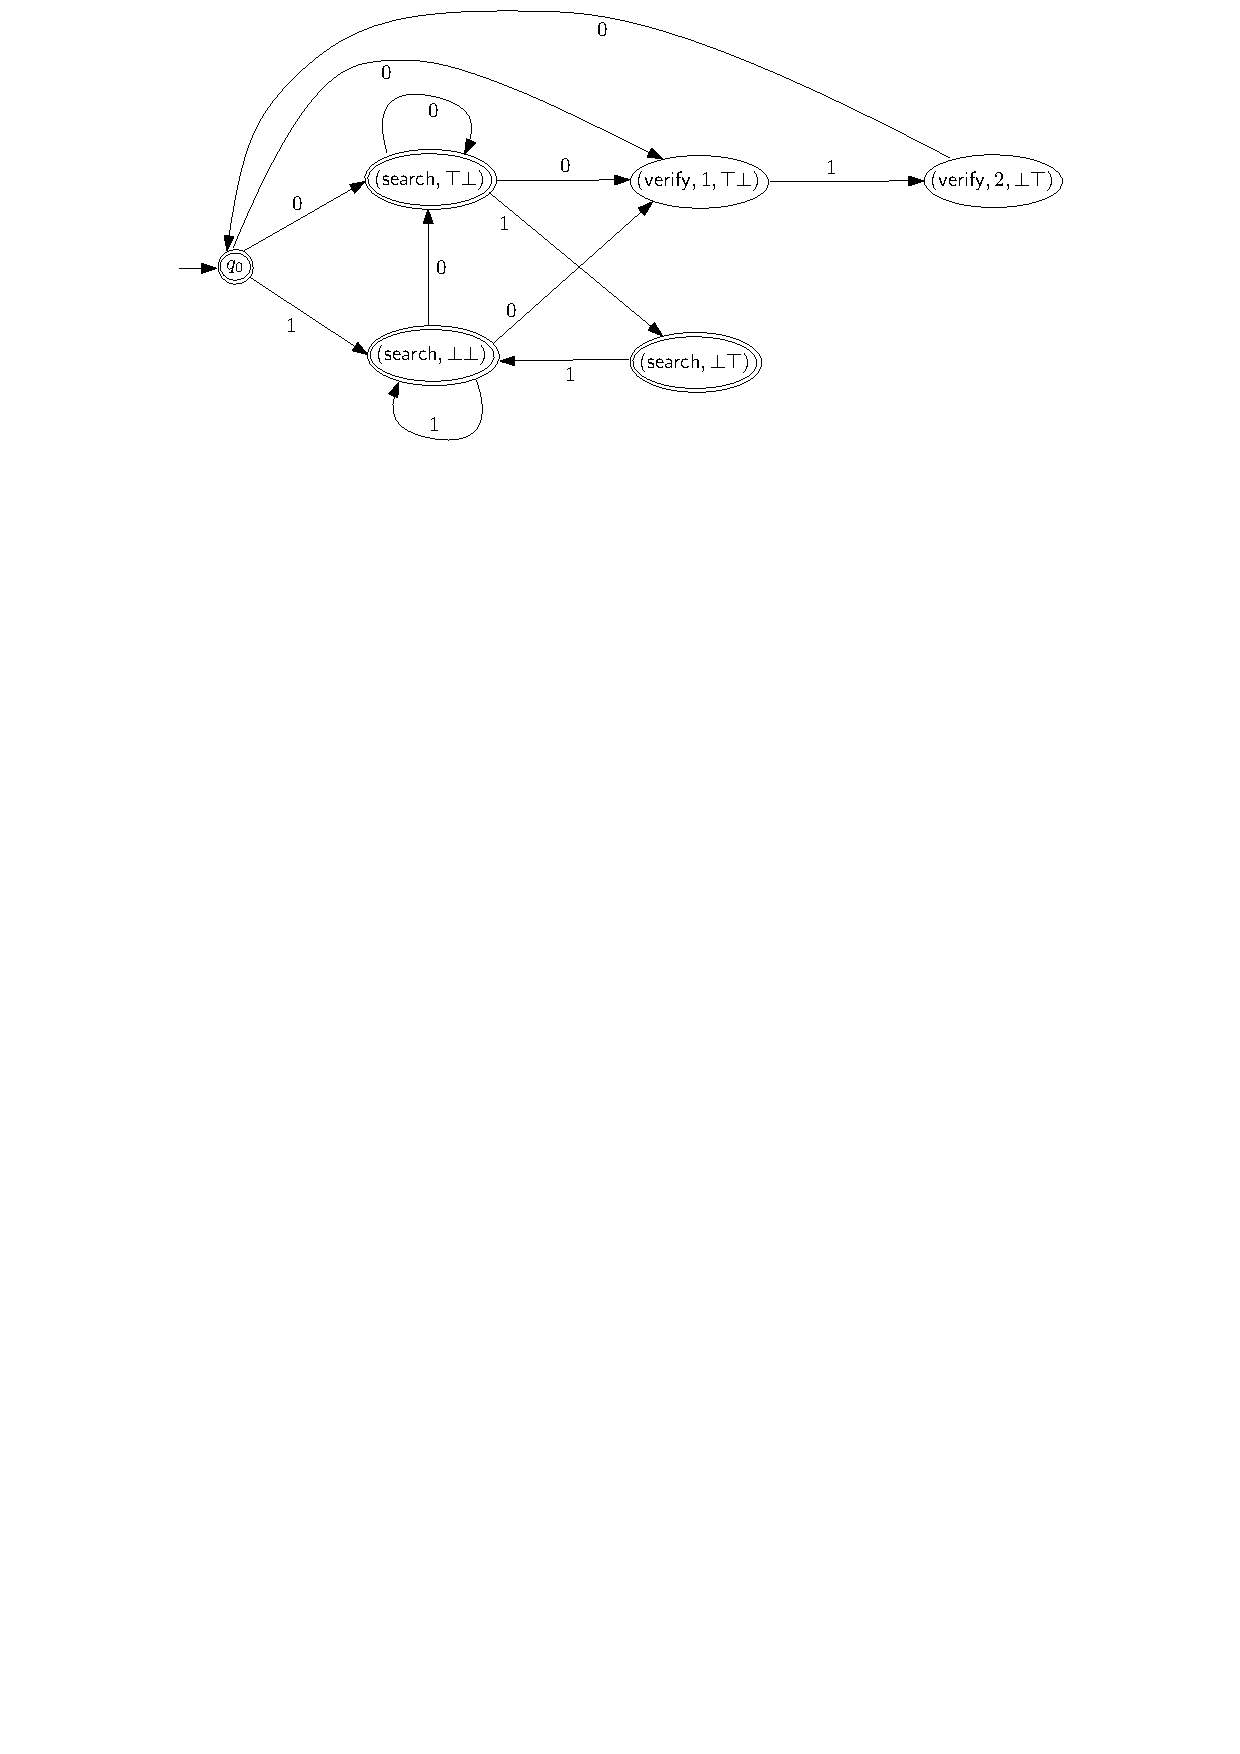
\includegraphics[scale=0.6]{parsing-automata-example.pdf}
\end{center}
\caption{The parsing automaton $\cA_u$ for $u = 010$}\label{fig-pa-exmp}
\end{figure}
\end{example}

We are ready to present the construction of $\cB_{\cA_1, u,  T_{z}}$. The NFA $\cB_{\cA_1, u, T_{z}}$ is constructed by the following three-step procedure.
\begin{enumerate}
\item Construct the product automaton $\cA_1 \times \cA_u$. Note that the initial state of $\cA_1 \times \cA_u$ is $(q_{0},q_0)$ and the set of final states of $\cA_1 \times \cA_u$ is $F_1 \times F_u$.

\item Remove from $\cA_1 \times \cA_u$ all the (incoming or outgoing) transitions associated with the states from $Q_1 \times Q_{\verify}$.

\item For each pair $(q,q') \in T_{z}$ and each sequence of transitions in $\cA_u$ of the form
$$
\begin{array}{l}
\left(p, u[1], \left(\verify, 1, \overrightarrow{W'_1} \right) \right), \left( \left(\verify, 1, \overrightarrow{W'_1} \right), u[2],
 \left(\verify, 2, \overrightarrow{W'_2}\right) \right), \\
 \hspace{3cm} \cdots, \left(\left(\verify, k-1, \overrightarrow{W'_{k-1}} \right), u[k], q_0\right),
\end{array}
$$
where  $p=q_0$ or $p = \left(\search, \overrightarrow{W} \right)$,
add the following transitions
$$
\begin{array}{c}
\left((q,p), u[1], \left(q, \left(\verify, 1, \overrightarrow{W'_1} \right) \right) \right), \\
\left( \left(q, \left(\verify, 1, \overrightarrow{W'_1} \right) \right), u[2], \left(q, \left(\verify, 2, \overrightarrow{W'_2}\right)\right)\right),  \\
\cdots, \\
\left(\left(q, \left(\verify, k-2, \overrightarrow{W'_{k-2}} \right) \right), u[k-1], \left (q, \left (\verify, k-1, \overrightarrow{W'_{k-1}} \right) \right) \right),\\ \left( \left(q, \left (\verify, k-1, \overrightarrow{W'_{k-1}} \right) \right), u[k], \left(q', q_0 \right)\right).
\end{array}
$$
Note that the number of aforementioned sequences of transitions in $\cA_u$ is at most $|Q_{\search}|+1$, since  $ \overrightarrow{W'_1},\dots,  \overrightarrow{W'_{k-1}}$ are completely determined by $\overrightarrow{W} $ and $u$.
Intuitively, when $\cA_u$ identifies an occurrence of $u$, if the current state of $\cA_1$ is $q$, then after reading the occurrence of $u$, $\cB_{\cA_1, u, T_z}$ jumps from $q$ to some state $q'$ such that $(q,q') \in T_z$.
\end{enumerate}

\begin{example}\label{exmp-cs-case}
Let us consider $C \equiv x = \replaceall(y, u, z) \wedge x \in e_1 \wedge y \in e_2 \wedge z \in e_3$, where $u = 010$, and $e_1,e_2,e_3$ are as in Example~\ref{exmp-sl} (cf. Figure~\ref{fig-sl-exmp}). The product automaton $\cA_1 \times \cA_u$ is illustrated in Figure~\ref{fig-cs-exmp}, where $\{q_2\} \times \cA_u$ denotes the automaton obtained from $\cA_u$ by changing each state $p$ in $\cA_u$ into $(q_2, p)$, similarly for $\{q_4\} \times \cA_u$. Let $T_z = \{(q_0,q_0),(q_1,q_2)\}$. Then the NFA $\cB_{\cA_1, u, T_z}$ is obtained from $\cA_1 \times \cA_u$ by first removing all the transitions  associated with the states from $Q_1 \times Q_{\verify}$, then adding the transitions according to $T_z$ as aforementioned (see Figure~\ref{fig-cs-exmp-2}, where the thick edges denote the added transitions).  It is a routine to check that $01010101$ is accepted by both $\cB_{\cA_1, u, T_z}$ and $\cA_2$. Moreover, $10 \in \Ll(\cA_3) \cap \Ll(\cA_1(q_0,q_0)) \cap \Ll(\cA_1(q_1,q_2))$. Let $y$ be $01010101$ and $z$ be $10$. Then $x$ takes the value $\replaceall(01010101, 010, 10)=101101$, which is accepted by $\cA_1$. Therefore, $C$ is satisfiable.
\begin{figure}[htbp]
\begin{center}
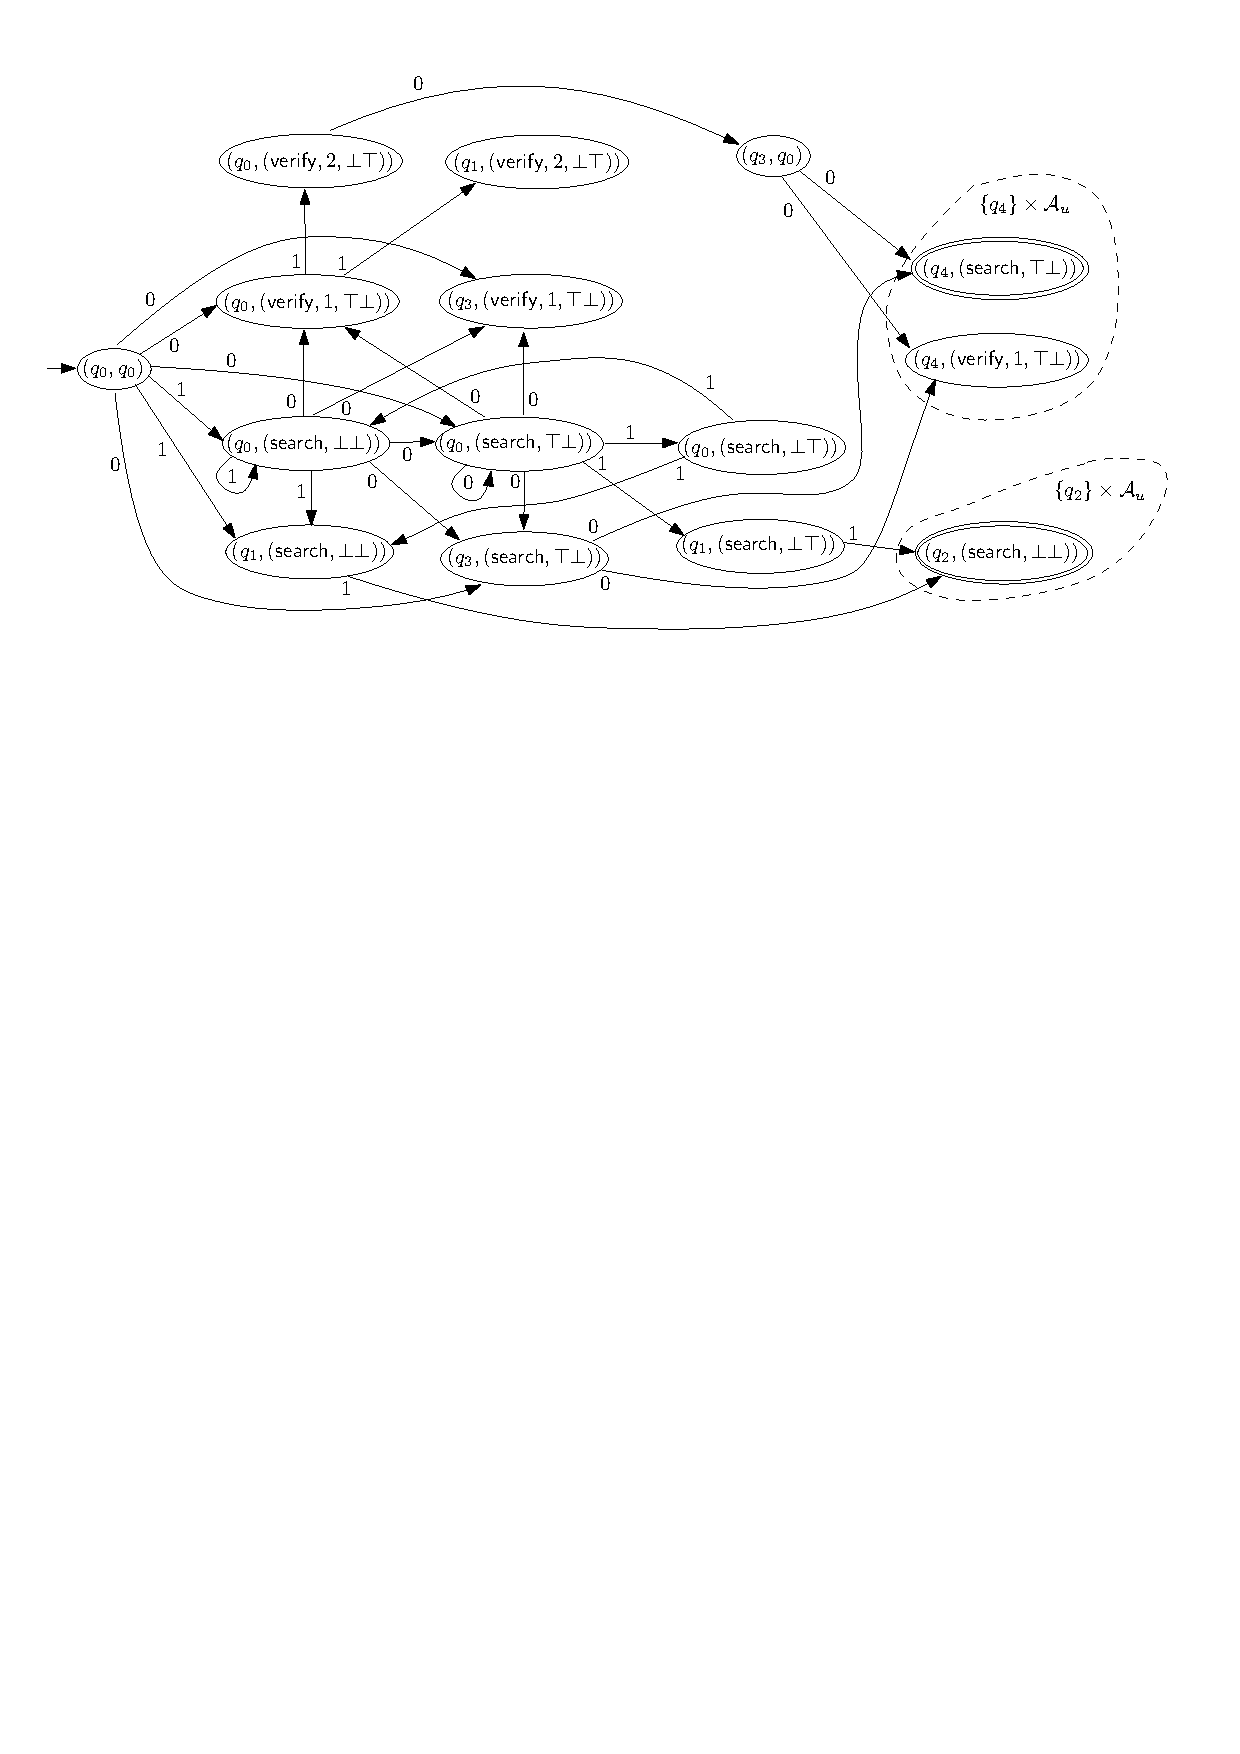
\includegraphics[scale=0.65]{constant-string-example.pdf}
\end{center}
\caption{The NFA $\cA_1 \times \cA_u$ for $u = 010$}\label{fig-cs-exmp}
\end{figure}
%
\begin{figure}[htbp]
\begin{center}
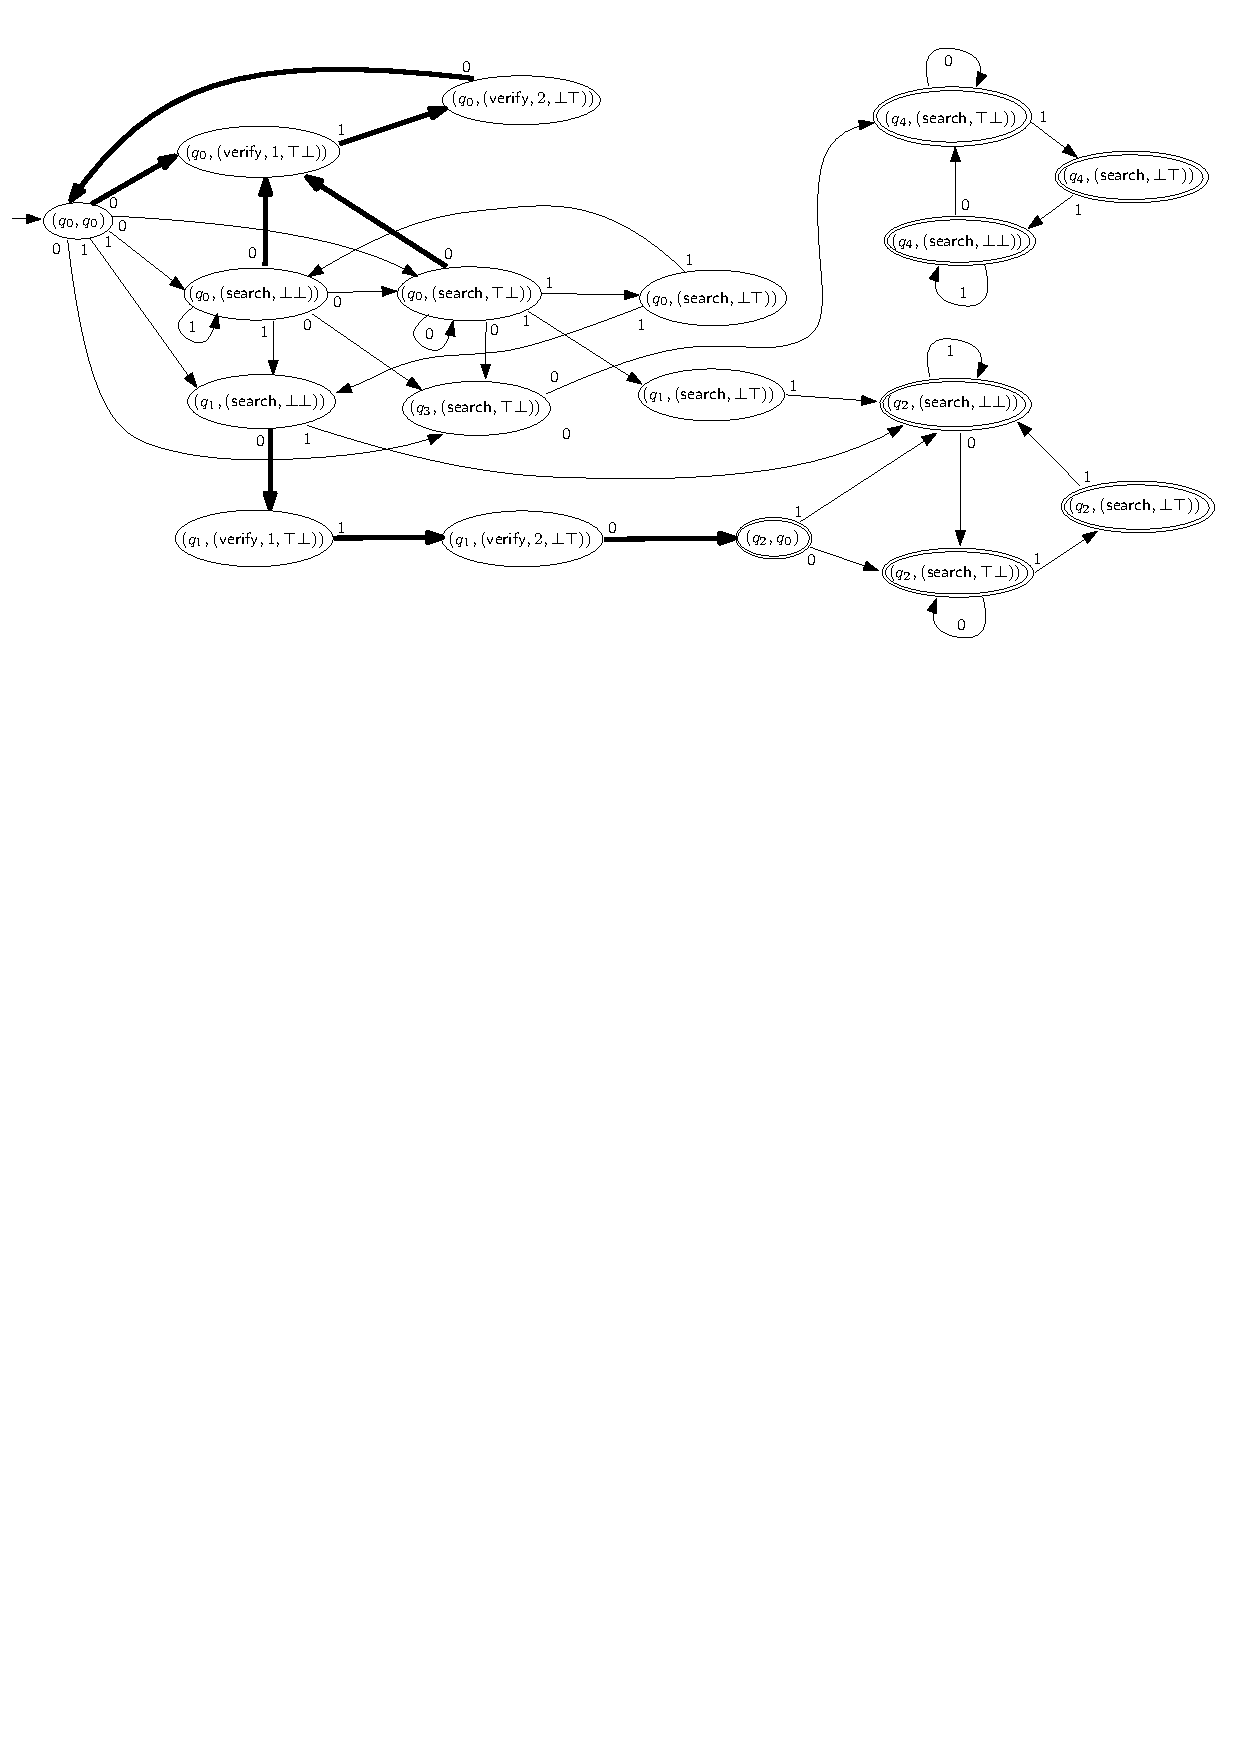
\includegraphics[scale=0.68]{constant-string-example-2.pdf}
\end{center}
\caption{The NFA $\cB_{\cA_1, u, T_z}$ for $u = 010$ and $T_z= \{(q_0,q_0),(q_1,q_2)\}$}\label{fig-cs-exmp-2}
\end{figure}
\end{example}

For the more general case that the $\strline[\replaceall]$ formula $C$ contains more than one occurrence of $\replaceall(\cdots)$ terms, similar to the single-letter case in Section~\ref{sec:replaceallsl}, we can nondeterministically remove the edges in the dependency graph $G_C$ in a top-down manner and reduce the satisfiability of $C$ to the satisfiability of a collection of regular constraints for source variables.

\paragraph*{Complexity}
When constructing $G_{i+1}$ from $G_i$, suppose the two edges from $x$ to $y$ and $z$ respectively are currently removed, let the labels of the two edges be $({\sf l}, u)$ and $({\sf r}, u)$ respectively, then each element $(\cT, \cP)$ of $\cE_i(x)$ may be transformed into an element $(\cT', \cP')$ of $\cE_{i+1}(y)$ such that $|\cT'| = O(|u||\cT|)$, meanwhile, it may also be transformed into an element $(\cT'', \cP'')$ of $\cE_{i+1}(z)$ such that $\cT''$ has the same state space as $\cT$.
%\mat{Also need to say the same about $z$?}\zhilin{the state space of the regular constraint for $z$ is not changed.}
Thus, for each source variable $x$, $\cE(x)$ contains at most exponentially many elements, and each of them may have a state space of at most exponential size. For instance, for a path from $x'$ to $x$ where the constant strings $u_1,\cdots, u_n$ occur in the labels of edges, an element $(\cT,\cP) \in \cE_0(x')$ may induce an element $(\cT', \cP')$ of $\cE(x)$ such that $|\cT'| \le |\cT| |u_1| \cdots |u_n|$, which is exponential in the worst case. 
%
To solve the nonemptiness problem of the intersection of all these regular constraints, the exponential space is sufficient. Consequently, in this case, we still obtain an EXPSPACE upper bound. 

Let us now consider the special situation that the $\rpleft$-length of $G_C$ is bounded by a constant $c$.
Since $\dmdidx(G_C) \le \lftlen(G_C)$, we know that $\dmdidx(G_C)$ is also bounded by $c$. Therefore, according to Proposition~\ref{prop-di}, there are at most polynomially different paths in $G_C$, we deduce that for each source variable $x$, $\cE(x)$ contains at most polynomially many elements. In addition, since the number of $\rpleft$-edges in each path is bounded by $c$, during the execution of the decision procedure, the number of times when $(\cT, \cP)$ of $\cE_i(x)$ may be transformed into an element $(\cT', \cP')$ of $\cE_{i+1}(y)$ such that $|\cT'| = O(|u||\cT|)$ is bounded by $c$.
Therefore, for each source variable $x$ and each element $(\cT'', \cP'')$ in $\cE(x)$,  $|\cT''|$ is at most polynomial in the size of $C$. We then conclude that for each source variable $x$, $\cE(x)$ corresponds to the intersection of polynomially many regular constraints such that each of them has a state space of polynomial size. Therefore, the nonemptiness of the intersection of all the regular constraints in $\cE(x)$ can be solved in polynomial space. In this situation, we obtain a PSPACE upper bound.

%Similarly to the single-letter case, we can define the dependency graph $G_C$. In addition, we can adapt $\dfs(z, z', a, f)$ into a procedure $\dfs(z, z', u, f)$, which integrates the automata $\cA_{u'}$ into the computation of the functions $f_{z', \cA_z}$, where $u,u'$ are constant strings occurring in the edge-labels in $G_C$.
